\documentclass[14pt]{extreport}

\usepackage[utf8]{inputenc}
\usepackage[italian,english]{babel}
\usepackage{graphicx}
\usepackage{cite}
\usepackage{amsmath}
\usepackage[table,xcdraw]{xcolor}
\usepackage{verbatim}
\usepackage{url}
\usepackage{listings}
\usepackage{comment}
\usepackage{hyperref}
%rimuove bordi dai link
\hypersetup{
    colorlinks=true,
    linkcolor=black,
    filecolor=magenta,      
    urlcolor=cyan,
}

\usepackage{fancyhdr}
\pagestyle{fancy}
\fancyhf{}
\setlength{\headheight}{17pt}
\rhead{Cap.\thechapter}
\fancyhead[L]{\rightmark}
\cfoot{\thepage}

\lstset{frame=tb,
	language=Java,
	numbers=left,
	keywordstyle=\color{blue},
	alsoletter={.}
}
\graphicspath{ {./Figure/} }

\usepackage{titlesec}

\titleformat{\chapter}{\normalfont\huge\bf}{\thechapter.}{20pt}{\huge\bf}
\titleformat{\section}{\normalfont}{\thesection.}{18pt}{\normalfont\bf}
\titleformat{\subsection}{\normalfont}{\thesubsection.}{16pt}{\normalfont\bf}



\begin{document}
\selectlanguage{italian}
\begin{titlepage}
\begin{center}
	\begin{figure}
    	
\includegraphics[width=1.5cm, height=1.5cm]{unisa.png}
    	\centering
    \end{figure}
	{\Large Università degli Studi di Salerno}\\[0.2truecm]
	{\large Dipartimento di Informatica\\Corso di Laurea Magistrale in Informatica}\\
	\hrulefill
	\vfill
	{\large Tesi di Laurea Magistrale in Informatica}\\[0.2truecm]
	%{\Large Informatica}\\
	\vfill\vfill
	{\LARGE {\bf Titolo}}
	
	\vfill\vfill
	
	
	\ \ \ \ \ \ \ {\bf Docente} \hfill {\bf Candidato}\ \ \\
	Prof.ssa \textbf{Delfina Malandrino} \hfill  \textbf{Francesco Vicidomini}
	\centerline{\hfill Matricola: 051210533}
	
	
	\vfill
	\hrulefill 
	\begin{center} Anno Accademico 2019-2020 \end{center}
	
\end{center}
\end{titlepage}

\setcounter{page}{1} 		
\pagenumbering{roman} 

\newpage
	
\newcommand{\quotes}[1]{``#1''}
\tableofcontents
\listoffigures %elenco figure
\listoftables %elenco tabelle
%%%%%%%%%%%%%%%%%%%%%%%%%%%%




%%%%%%%%%%%%%%%%%%%%%%%%%%%%
\chapter*{Abstract}
 
Gli Online Social Network(OSN) sono tra le applicazioni che hanno maggiore utenza e posseggono gran parte dei dati personali dei loro utenti.\newline
La gestione dei dati personali da parte di questi colossi dell'IT viene regolata attraverso apposite leggi, ma spesso sono gli utenti stessi a pubblicare involontariamente delle informazioni sensibili che possono esporli a dei rischi. Ad esempio abbiamo sentito spesso parlare di furti in appartamento fatti proprio perché i ladri avevano visto sui social delle vittime che queste erano partite per una vacanza.\newline
L'obiettivo di questa tesi è aggiungere al plugin di Chrome Knoxly la possibilità di riconoscere dati sensibili in base al contesto in cui sono stati scritti e in base a quanto l'utente reputi sensibili questi dati. Per raggiungere questo obiettivo è stata sviluppata e installata all'interno di Knoxly una intelligenza artificiale in grado di riconoscere il dato sensibile estrapolandolo dalla semantica della frase in cui viene menzionato, in seguito l'utente indicherà quanto questo dato sia sensibile per egli. Ad esempio se il proprietario di una pasticceria tweetta "Ho una pasticceria in via Roma" l'indirizzo viena riconoscito come un dato sensibile ma per il pasticciere questo non lo è perchè sta usando quel tweet per farsi pubblicità quindi egli comunicherà al sistema che per lui quel dato non è sensibile e il sistema aggiornerà la sua IA.


%%%%%%%%%%%%%%%%%%%%%%%%%%%%

%%%%%%%%%%%%%%%%%%%%%%%%%%%%
\chapter{Introduzione}
\setcounter{page}{1} 		
\pagenumbering{arabic}
\section{Contesto}
Da una decina d'anni a questa parte gli OSN sono sempre più presenti nella vita di milioni di persone; siamo arrivati al punto che una singola persona possiede anche più tipi di social network (o addirittura account multipli) e su ognuno di questi, spesso sulla base del tipo di comunicazione che permette, pubblica contenuti diversi. I social network incoraggiano sostanzialmente gli utenti a condividere più o meno la loro privacy per migliorare la loro presenza nel mondo virtuale. Questo fa si che su queste piattaforme viaggi una enorme mole di informazioni.

In particolare, alcuni studi dimostrano che gli utenti a volte rivelano troppe informazioni o divulgano involontariamente messaggi che minano la loro privacy, specialmente quando sono negligenti, emotivi o inconsapevoli dei rischi~\cite{looseTweets, studyFb, readMyTwitter}.
Per la maggior parte degli utenti, i loro post sono pensati solo per essere condivisi con amici / follower, ma il pubblico degli OSN è significativamente più grande delle aspettative degli utenti, tra cui inserzionisti, recruiter, robot dei motori di ricerca, ecc.
Spesso queste informazioni pubblicate sugli OSN possono contenere informazioni sensibili e/o personali proprie o di terzi. 

Quando gli utenti di un OSN si registrano ad esso questi stanno affidando alla piattaforma alla quale si iscrivono la loro anagrafica e molte altre informazioni che possono contribuire alla identificazione univoca di se stessi. A gestori degli OSN viene affidato il compito di manutenere e di tenere al sicuro i dati che l'utente gli affida. Purtroppo sono stati riportati dei casi in cui delle falle di sicurezza presenti in alcuni OSN abbiano portato al furto di molti account (e ai dati ad esso connessi).

Pertanto, c'è la necessità di poter identificare contenuti online potenzialmente sensibili, in modo che gli utenti possano essere avvisati di tali minacce ed agire di conseguenza prima che il contenuto venga pubblicato in rete.

%A tal proposito è stato dimostrato, che su una sessione di navigazione che comprendeva un insieme di azioni tipiche di un utente (accesso a social network, ricerche, posting di commenti, ecc), Google Analytics raccoglieva circa l’87\% dei dati personali e sensibili disponibili~\cite{MalandrinoScarano}.



\subsection{Alcuni casi di furto di informazioni}
\label{ssec:exampleLeak}
\textbf{1. AOL search data leak}\cite{aolDataLeak}\newline
Nel 2006 la compagnia internet AOL pubblica un grande numero di ricerche fatte dagli utenti. Le ricerche pubblicate da AOL erano anonime ma, molte di queste, contenevano informazioni personali sensibili.

Partendo da queste ricerche, il \textit{New York Times} è stato in grado di risalire a molte delle persone che avevano effettuato quelle ricerche.\newline
\textbf{2. Myspace account leakage}\cite{myspacebreach}\newline
Nel 2016 sono stati trovati 360 milioni di account myspace in vendita sul deep web. I dati comprendevamo mail, password, username di una parte degli utenti create prima del giugno 2013.\newline
\textbf{3. Cambridge Analytica}\cite{cambridge}\newline
Nel 2018 viene rivelato che la società di consulenza politica Cambridge Analytica aveva raccolto i dati di milioni di utenti Facebook e li ha usati per scopi di propaganda politica.

I dati raccolti da Cambridge Analytica sono stati utilizzati per la campagna elettorale di Donald Trump, Brexit, e le elezioni messicane del 2018.\newline
\textbf{4. Caso Renzi Formigli}\cite{formigli}\newline
In questo caso non c'è un colosso della IT che per una falla di sicurezza perde le informazioni sensibili dei sui utenti ma una persona che rivela in maniera indiretta dati sensibili di una terza.

Il giornalista e conduttore televisiovo Corrado Formigli intervista il senatore della Repubblica Matteo Renzi in merito al prestito che gli era stato fatto da un suo amico per l’acquisto di una villa.


Durante la trasmissione il conduttore mostra le foto della villa, poche ore dopo il termine della trasmissione su Facebook compaiono post che parlano e mostrano la casa del giornalista.

\section{Privacy leakage}
\label{sec:privacyLeakage}
Nella sezione \ref{ssec:exampleLeak} sono stati illustrati alcuni esempi di \textbf{privacy leakage}, ovvero, contenuti sensibili o inappropriati che gli utenti stessi, inconsapevolmente o involontariamente, divulgano durante l'utilizzo dei social o altri servizi (es. e-mail).I contenuti possono riguardare la propria vita privata o quella altrui.

\section{Norme per tutelare la privacy degli utenti}
Per migliorare e regolamentare la gestione dei dati sensibili e personali sul web la Commissione Europea ha iniziato ad aggiornare le regole in ambito privacy dal 2016, concentrandosi sul controllo della diffusione dei dati e sul conoscere da \textit{chi} e \textit{come}, questi vengano trattati.

La normativa europea GDPR(General Data Protection Regulation)\footnote{https://gdpr-info.eu/} definisce come \textit{dati personali} le informazioni che identificano o rendono identificabile, direttamente o indirettamente, una persona fisica e che possono fornire informazioni sulle sue caratteristiche, le sue abitudini, il suo stile di vita le sue relazioni personali, il suo stato di salute, la sua situazione economica, ecc.

Il GDPR quindi riduce il rischio di uso improprio e violazioni della privacy,
causate intenzionalmente o per mancanza di consapevolezza.

Inoltre la Convenzione 108\footnote{https://www.coe.int/en/web/data-protection/convention108/modernised} e il Regolamento Europeo prevedono che i dati devono
essere conservati per un periodo di tempo limitato, e in particolare non
oltre il tempo necessario per raggiungere lo scopo alla base del trattamento.
Nel caso in cui un titolare del trattamento volesse mantenerli per un periodo
superiore, deve procedere alla loro anonimizzazione.

\section{Cos'è Knoxly}
\label{sec:whoisKnoxly}
Knoxly (Figura \ref{fig:logoKnoxly}) si prefigge come obiettivo quello di aiutare gli utenti ad avere una maggiore consapevolezza
dei dati che pubblicano/condividono sul Web , dato che il principale rischio per la privacy online è la divulgazione di
informazioni personali e sensibili degli stessi utenti.\newline
\begin{figure}[h]
    \centering
    
\includegraphics[scale=0.25]{Figure/logoKnoxly.png}
    \caption{logo di Knoxly}
    \label{fig:logoKnoxly}
\end{figure}
\FloatBarrier
Spesso gli utenti degli OSN divulgano anche senza la piena consapevolezza dati sensibili e/o personali proprio o di terzi. A tal fine, Knoxly (1) individua quali dati sensibili e personali sono presenti in un messaggio di testo che l’utente è intenzionato a pubblicare/condividere sul Web, (2) li mostra attraverso un’ interfaccia grafica user-friendly e (3) lascia all’utente decidere quali o quante informazioni sensibili e personali è disposto a condividere con la divulgazione di tale messaggio.

A differenza dei convenzionali meccanismi di protezione della privacy sui dati o sui OSN, che si focalizzano principalmente sulla protezione dell’identità o di attributi privati \cite{collective-data, diff-privacy, urwho, inferr-privacy, protection-private, stalking}, Knoxly si muove verso l’idea di \quotes{\textit{privacy as having the ability to control the dissemination of sensitive information}}.

Attualmente i limiti di Knoxly sono quelli intrinsechi ad una analisi lessicale. Per questa ragione, in questo lavoro ci si vuole muovere verso metodi intelligenti che oltrepassino i metodi keyword-based, aggiungendo un \quotes{modulo semantico} in grado di capire se un testo scritto da un utente contenga o meno dati sensibili e/o personali.

\section{Il modello di minaccia}
Knoxly mira a proteggere gli utenti del Web dalla diffusione accidentale di qualsiasi contenuto inappropriato, in particolare le informazioni private o sensibili su se stessi. Si considera principalmente il rischio di una diffusione inappropriata a due tipo di pubblico: (1) follower o amici, che ricevono aggiornamenti dei post dell'utente; (2) staker esterni, che sbirciano nei post dei social network di un utente target. È probabile che entrambi conoscano l'identità offline dell'utente. Knoxly non impedisce all'utente di pubblicare i contenuti(sensibili) nè impedisce al destinatario di visualizzare i contenuti, fornendo privacy awareness. L'idea di Knoxly parte dal presupposto che dei tracciatori possono esplorare l'OSN attraverso l'interfaccia utente o raccogliere dati utilizzando un crawler automatizzato tramite l'API dell'OSN di riferimento. Infine, non considera la retrazione/cancellazione dei post precedenti, nè li analizza.

\section{Obiettivi del lavoro}
Questo lavoro si prefigge l'obiettivo di aggiungere a Knoxly un modulo intelligente in grado di poter riconoscere un dato sensibile in un testo scritto in linguaggio naturale senza affidarsi a meccanismi keyword-based, di segnalare all'utente la presenza di questo dato e di dare la possibilità all'utente di personalizzare il livello delle segnalazioni in modo tale che esso possa \quotes{imparare} a riconoscere quali sono i dati sensibili secondo lo specifico l'utente che sta utilizzando il plugin.

\subsection{I dati sensibili}
\label{ssec:sensitive_data}
Nelle precedenti sezioni si è molto discusso di dati sensibili, ma cosa sono esattamente? Secondo la normativa GDPR attualmente in vigore per dati sensibili si intendono i dati che rivelino:
\begin{itemize}
    \item l'etnia, pensiero politico, religioso o filosofico
    \item se si è membri di un sindacato
    \item dati genetici o biomedici che permettano l'identificazione univoca di un essere umano
    \item dati relativi alla salute
    \item orientamento sessuale e vita sessuale
\end{itemize}
Abbiamo scelto di utilizzare un sottoinsieme di temi di partenza per dare una conoscenza di base all'IA di Knoxly. L'IA inizialmente sarà in grado di individuare dati sensibili riguardo i seguenti topic
\begin{enumerate}
    \item orientamento politico
    \item salute
    \item lavoro
    \item viaggi
\end{enumerate}
Questi temi sono stati scelti per due motivi: (a) molti di questi temi fanno parte della normativa GDPR quindi è una legge a dirci che i dati appartenenti a quelle categorie sono sensibili e (b) molti dei temi che verranno trattati sono già stati utilizzati in vari riguardanti la privacy detection e il privacy leakage~\cite{looseTweets, MalandrinoScarano, dontTweetThis}.

%%%%%%%%%%%%%%%%%%%%%%%%%%%%
\chapter{I dati}
In questo capitolo si descrivono i metodi di machine learning utilizzati in questo lavoro (Sezione~\ref{sec:models}), quali metriche sono state utilizzate per misurarne le performance (Sezione~\ref{metrics}) ed infine si mostra una paronamica sulle tecniche di embedding focalizzando l'attenzione sul sentence embedding, una tecnologia emergente negli ultimi 5 anni (Sezione~\ref{sec:use}).

\section{Modelli utilizzati}
\label{sec:models}
\subsection{Random Forest}
\label{ssec:RF}
Il Random Forest(RF) è un algoritmo di supervised classification che consiste in un insieme di metodi basati sul bagging\cite{Random Forest}; è stata usata l'implementazione di \textit{scikit-learn} che combina gli alberi facendo la media della loro previsione probabilistica invece di lasciare che ogni albero voti per una singola classe, e supporta intrinsecamente problemi multi-classe come quelli che vedremo nel Capitolo~\ref{ch:method}.

%\subsection{Support Vector Machine}
%\label{ssec:SVM}

%\subsection{MultiLayer Perceptron}
%\label{ssec:MLP}
\section{Metriche per valutazione delle performance}
\label{metrics}
Esistono diverse metriche per valutare i punteggi dei modelli di machine learning. In questo lavoro sono state utilizzate le seguenti metriche:

\begin{itemize}
    \item \textbf{accuracy}: frazione delle predizioni corretta fatte dal nostro modello, essa è definita come segue
    \begin{equation*} accuracy = \dfrac {(tp + tn)}{(tp + tn + fp + fn)}\end{equation*} 
    dove $tp$, $fn$, $fp$ e $tn$ sono rispettivamente il numero di veri positivi, falsi negativi, falsi positivi, veri negativi
    
    \item \textbf{precision}: capacità del classificatore di non etichettare come positivo un campione che è negativo, definita come segue
    \begin{equation*} precision = \dfrac {tp}{(tp + fp)}\end{equation*} 
    dove $tp$ rappresenta il numero di veri positivi e $fp$ il numero di falsi positivi
    
    \item \textbf{recall}: capacità di un classificatore di trovare tutti i campioni positivi; definita come
    \begin{equation*} recall = \dfrac {tp}{(tp + fn)}\end{equation*} 
    dove $tp$ rappresenta il numero di veri positivi e $fn$ il numero di falsi negativi
    
    \item \textbf{F1-score}: è la media armonica di precision e recall. Varia tra 0 e 1, dove 0 è il peggior punteggio possibile e 1 il migliore. Spesso si utilizza quando si ha a che fare con problemi multi-classe (non binari). La formula per il punteggio F1 è:
    \begin{equation}
       F_1score = 2 * \frac{(precision * recall)}{(precision + recall)}
    \end{equation}
    possiamo dire di avere un buon classificatore quando abbiamo una alta accuracy e una bassa recall
    \item \textbf{roc-auc}: l'AUC rappresenta l'area sotto la curva (Area Under the Curve) ROC (Receiver Operating Characteristic)~\cite{RocAUC}. La curva ROC, il modo più comune per valutare le performance di classificatori binari, è creata tracciando su di un piano cartesiano i veri positivi e i falsi positivi. I valori di roc auc variano tra 0 e 1, dove 1 rappresenta il classificatore perfetto.
\end{itemize}

\section{Tecniche di embedding per NLP}
\label{sec:use}
Nell'ambito del'Natural Language Processing sono state introdotte diverse tecniche per comprendere il significato di una parola o di una frase con lo scopo di rispondere a delle domande ~\cite{wu2017visual} alla sentiment analysis ~\cite{kaur2017survey} e altro ancora.

Negli ultimi anni, il word embedding si è affermato come uno dei metodi di rappresentazione più popolari~\cite{bengio2003neural,collobert2008unified,turian2010word}.
La sua capacità sta nel fatto di sapere cogliere il contesto di una parola in un documento , la somiglianza semantica e sintattica, la relazione con altre parole, ecc. La tecnica più popolare in questo campo è la {\tt Word2vec}, presentata in ~\cite{mikolov2013efficient,mikolov2013distributed} ma sono state introdotte anche altre tecniche come {\tt SkipGram}, {\tt CBOW}, {\tt Log-Bilinear language}~\cite{mnih2007three} ecc. Essi usano un oggetto simile alla probabilità condizionale $P(w|c)$, che prevede la parola target $w$ in base al suo contesto $c$. Sono stati utilizzati per una varietà di compiti, ad esempio, l'estrazione di testi legati alla finanza~\cite{wang2019user}, question answering~\cite{yang2019online}.

Il successo dei metodi di rete neurale per il calcolo del word embedding ha motivato i metodi per la generazione di embedding semantici di testi più lunghi, come frasi e paragrafi. Sono metodi per fare embed di una frase completa in uno spazio vettoriale n-dimensionale. I sentence embed ereditano alcune proprietà dai word embed~\cite{arora2016simple}.

Quindi si potrebbe usare l'embed delle frasi per diversi scopi:
\begin{enumerate}
    \item calcolare la matrice di similarità delle frasi basandosi sugli embed
    \item tracciare frasi con una tecnica di mappatura comune
    \item predict some value for the sentence, ad esempio, sentimento espresso nella frase.
\end{enumerate}
Una applicazione del sentence embedding può essere vista inn~\cite{iyyer2015deep}, dove gli autori usano sentence embeddings in sentiment analysis e question answering. In questo campo, un'enorme tendenza è la ricerca degli Universal Embeddings: embeddings che sono pre-addestrati su un grande corpus e possono essere inseriti in una varietà di modelli di compiti a valle (sentimental analysis, classification, translation) per migliorare automaticamente le loro prestazioni incorporando alcune rappresentazioni generali di parole/frasi apprese sul più ampio dataset.

{\tt FastText}~\cite{joulin2016fasttext}, definito e sviluppato dagli stessi autori di {\tt Word2vec}, ha innescato l'esposione della ricerca sullo universal word embeddings. Il miglioramento principale di {\tt FastText} sull'originale {\tt Word2vec} è l'inclusione di n-grammi, che permettono di calcolare le rappresentazioni delle parole per le parole che non sono apparse nei dati di formazione (parole \quotes{fuori dal vocabolario}).

In questo senso, Google ha sviluppato un proprio sentence embedder, chiamato {\tt Universal Sentence Encoder}, che è in grado di gestire un gran numero di compiti nell'elaborazione del linguaggio naturale~\cite{USE}. In primo luogo, lo hanno sviluppato in lingua inglese, e in secondo luogo, hanno ampliato tale metodo per la contabilità di più di dieci lingue, tra cui italiano, tedesco, spagnolo, ecc~\cite{yang2019multilingue}, e lo hanno reso disponibile su Tensorflow Hub\footnote{\url{https://bit.ly/36BSS52}}. Questa versione multilingua effettua l'embed del testo da 16 lingue (arabo, cinese-semplificato, cinese-tradizionale, francese, inglese, italiano, giapponese, coreano, olandese, polacco, portoghese, spagnolo, tailandese, turco, russo, tedesco) in un unico spazio semantico utilizzando un doppio encoder multitasking addestrato che impara le rappresentazioni legate utilizzando, a sua volta, compiti di bridge basati sulla traduzione. L'Universal Sentence Encoder ha dimostrato di mostrare buone prestazioni con una quantità minima di allenamento supervisionato~\cite{USE}; prende in input un testo di lunghezza variabile, e l'uscita è un vettore di 512 dimensioni. 

Questo encoder può essere usato per task di text classification, semantic similarity, clustering e altri task riguardanti l'ambito dell'analisi del testo scritto in linguaggio naturale.\newline
In Figura~\ref{fig:my_label} viene mostrato il funzionamento di USE, egli prende in input un testo scritto in linguaggio naturale, codifica la frase in un array di 512 numeri reali, infine è stata misurata la similarità semantica delle frasi codificate utilizzando l'inner product tra gli embed. La similarità $s \in [0..1]$ è tanto più alta quanto più simili le frasi. 
\begin{figure}[h]
    \centering
    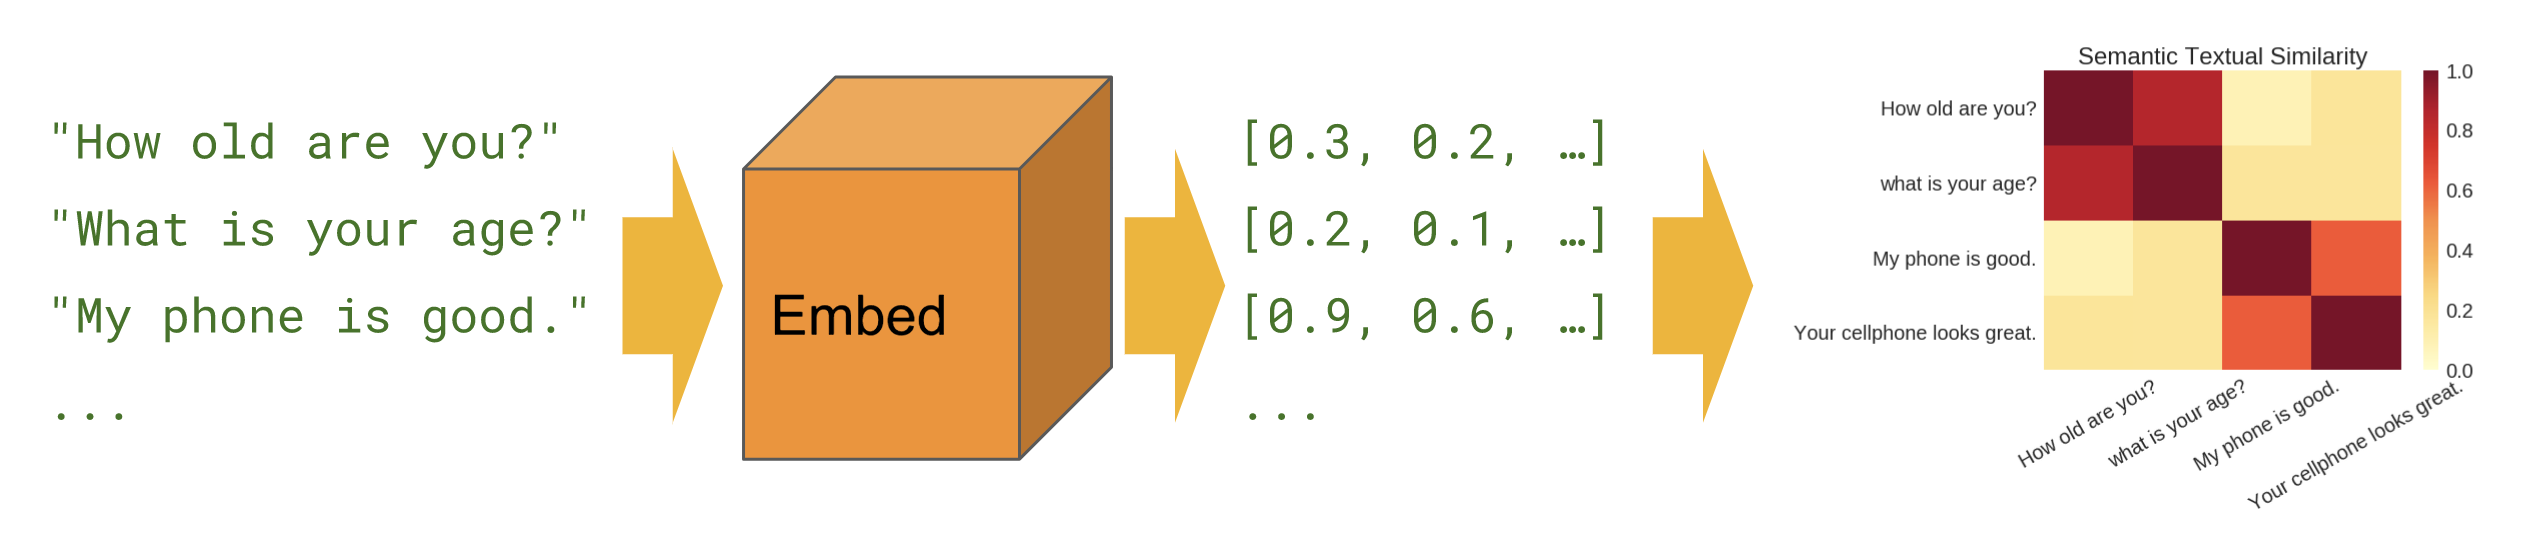
\includegraphics [scale=0.33]{Figure/use.png}
    \caption{Esempio funzionamento Universal Sentence Encoder: le frasi vengono trasformate in vettori a lunghezza fissa, per valutarne la similarità si può banalmente calcolare l'inner-product di tutte le coppie e mostrarlo in una matrice.}
    \label{fig:my_label}
\end{figure}
\FloatBarrier
In questo lavoro, è stato usato il multilingual Universal Sentence Encoder per effettuare l'embedding di frasi scritte in linguaggio naturale al fine di addestrare un classificatori in grado di riconoscere i topic a cui appartiene la frase e dei classificatori in grado di riconoscere la sensibilità della frase appartenente al topic.

%\chapter{Titolo capitolo}
%Qui ci va quell'articolo che abbiamo trovato su PET passo passo illustrato, e sottolineato i pregi/difetti.

\begin{thebibliography}{9}
\bibitem{looseTweets} 
Huina Mao, Xin Shuaiand Apu Kapadia.\newline
\textit{Loose Tweets: An Analysis of Privacy Leaks on Twitter}. \newline
WPES 2011.

\bibitem{privacyDetective}
Aylin Caliskan, Jonathan Walsh, Rachel Greenstadt.\newline
\textit{Privacy Detective: Detecting Private Information and Collective Privacy Behavior in a Large Social Network}.\newline
WPES 2014

\bibitem{dontTweetThis}
Qiaozhi Wang, Hao Xue, Fengjun Li, Dongwon Lee, and Bo Luo.\newline
\textit{\#DontTweetThis: Scoring Private Information in Social Networks}. \newline
POPETS 2019
\end{thebibliography}

\end{document}